\documentclass[border=3pt]{standalone}
% Preâmbulo compartilhado pelos diagramas TikZ da aula 5 de IHC (Processos de Design)
\usepackage[T1]{fontenc}
\usepackage[utf8]{inputenc}
\usepackage{lmodern}
\usepackage{amsmath}
\usepackage{xcolor}
\usepackage{tikz}
\usetikzlibrary{arrows.meta,angles,quotes,decorations.pathmorphing,calc,
                positioning,shapes.geometric,shapes.misc,backgrounds,fit,
                math}

% Paleta (mesma dos SVGs originais)
% Paleta da disciplina de IHC: acento roxo (#755099), da capa do livro.
% (o nome "dblue" é mantido para não alterar todos os diagramas)
\definecolor{dblue}{HTML}{755099}
\definecolor{dorange}{HTML}{B3541E}
\definecolor{dgreen}{HTML}{4A7C59}
\definecolor{dred}{HTML}{9C4B4B}
\definecolor{dcream}{HTML}{F4F1EA}
\definecolor{dshade}{HTML}{DDD7C9}

% Função gaussiana (não normalizada por padrão de escala visual)
\pgfmathdeclarefunction{gauss}{3}{%
  \pgfmathparse{1/(#3*sqrt(2*pi))*exp(-((#1-#2)^2)/(2*#3^2))}%
}

% Estilos comuns (prefixo d... para não colidir com chaves internas do pgf)
\tikzset{
  >={Stealth[length=2mm]},
  dguide/.style={gray!55, dashed, line width=0.4pt},
  daxis/.style={gray!60, line width=0.7pt, ->},
  dbody/.style={fill=black!3, draw=black!80, line width=1pt},
  dacc/.style={draw=dblue, line width=1pt},
  dlbl/.style={black!55, font=\small},
  dsub/.style={black!45, font=\footnotesize},
  dstate/.style={circle, draw=black!80, fill=dcream, line width=1pt,
                 minimum size=17mm, font=\large, inner sep=1pt},
  dobs/.style={circle, draw=black!80, fill=dshade, line width=1pt,
               minimum size=14mm, font=\large, inner sep=1pt},
  dbox/.style={rounded corners=2pt, draw=black!80, fill=dcream, line width=1pt,
               align=center, inner sep=6pt},
  dop/.style={circle, draw=black!80, fill=white, line width=1pt,
              minimum size=6mm, inner sep=0pt, font=\small},
  dtrans/.style={->, dblue, line width=1pt},
  dmeas/.style={->, dorange, line width=1pt},
  dcurve/.style={line width=1pt, dblue},
  dcurveb/.style={line width=1.4pt, dorange},
}

\begin{document}
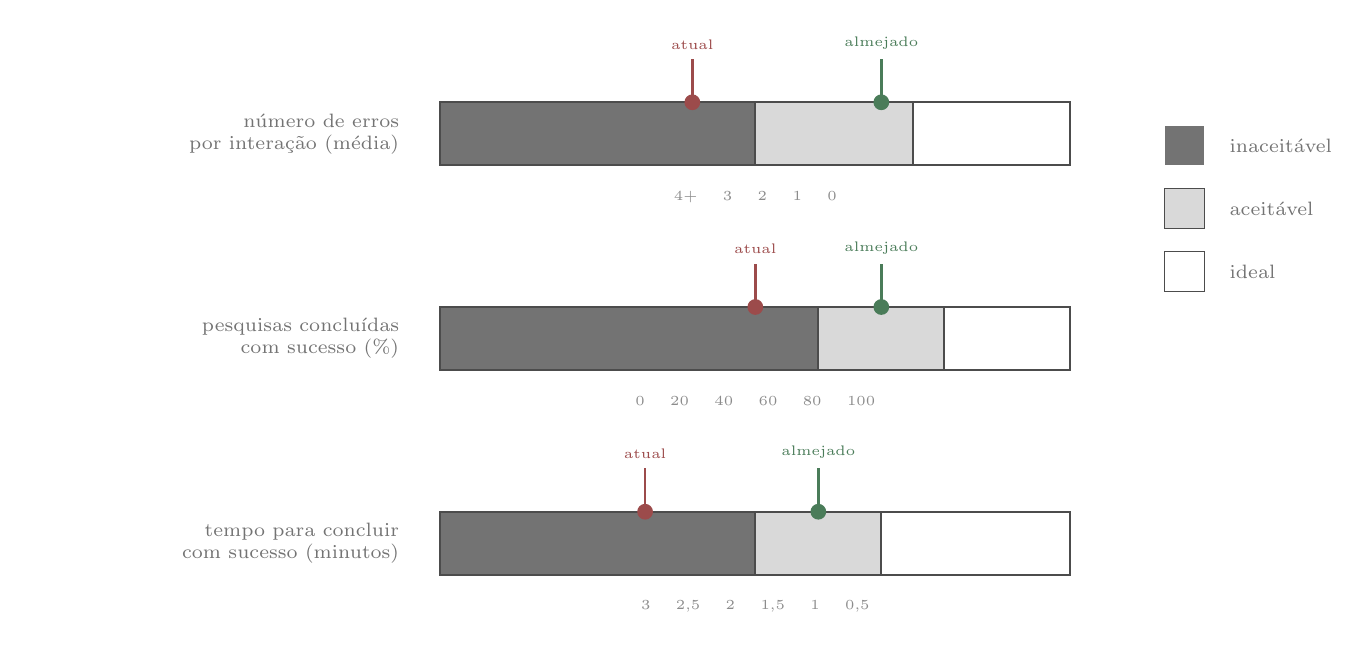
\begin{tikzpicture}[x=1cm,y=1cm]

  % args: y  inaceitavel-aceitavel(x)  aceitavel-ideal(x)  rotulo  atual  almejado  ticks
  \newcommand{\barra}[7]{%
    \begin{scope}[shift={(0,#1)}]
      \node[dlbl, font=\scriptsize, anchor=east, text width=4.6cm, align=right] at (-0.4,0.4) {#4};
      \fill[black!55] (0,0) rectangle (#2,0.8);
      \fill[black!15] (#2,0) rectangle (#3,0.8);
      \fill[white] (#3,0) rectangle (8,0.8);
      \draw[black!70, line width=0.7pt] (0,0) rectangle (8,0.8);
      \draw[black!70, line width=0.7pt] (#2,0) -- (#2,0.8) (#3,0) -- (#3,0.8);
      \draw[dred, line width=0.9pt] (#5,0.8) -- (#5,1.35); \fill[dred] (#5,0.8) circle (0.1);
      \node[dred, font=\tiny, anchor=south] at (#5,1.35) {atual};
      \draw[dgreen, line width=0.9pt] (#6,0.8) -- (#6,1.35); \fill[dgreen] (#6,0.8) circle (0.1);
      \node[dgreen, font=\tiny, anchor=south] at (#6,1.35) {almejado};
      \node[dsub, font=\tiny] at (4,-0.4) {#7};
    \end{scope}}

  \barra{5.2}{4.0}{6.0}{número de erros\\por interação (média)}{3.2}{5.6}{4+ \quad 3 \quad 2 \quad 1 \quad 0}
  \barra{2.6}{4.8}{6.4}{pesquisas concluídas\\com sucesso (\%)}{4.0}{5.6}{0 \quad 20 \quad 40 \quad 60 \quad 80 \quad 100}
  \barra{0}{4.0}{5.6}{tempo para concluir\\com sucesso (minutos)}{2.6}{4.8}{3 \quad 2,5 \quad 2 \quad 1,5 \quad 1 \quad 0,5}

  \fill[black!55] (9.2,5.2) rectangle (9.7,5.7); \node[dlbl, font=\scriptsize, anchor=west] at (9.9,5.45) {inaceitável};
  \fill[black!15] (9.2,4.4) rectangle (9.7,4.9); \draw[black!70] (9.2,4.4) rectangle (9.7,4.9); \node[dlbl, font=\scriptsize, anchor=west] at (9.9,4.65) {aceitável};
  \fill[white] (9.2,3.6) rectangle (9.7,4.1); \draw[black!70] (9.2,3.6) rectangle (9.7,4.1); \node[dlbl, font=\scriptsize, anchor=west] at (9.9,3.85) {ideal};

\end{tikzpicture}
\end{document}
